



Die Grundlegende Idee bestand darin eine Frequenzanalyse mit Wavelets zu machen. Diese kann dann verwendet werden um die Signale nach belieben zu manipulieren und nach wünschen anzupassen. Die Multiskalenanalyse bietet einen schnellen Rechenalgorhytmus jedoch ist er darauf konzipiert keine redundate Daten zu erzeugen. Durch das prinzip der Frequenzhalbierung, die auf jedem sogenannten Level einer Multiskalenanalyse passiert, sieht man nur alle Oktaven eines Signales. So können Frequenzen die nahe bei einander liegen nicht von einander unterschieden werden. Dafür lässt sich das ursprüngliche Signal nach einer msa wieder verlustfrei rekonstruieren. 

\subsection{Framing}
Die normale msa besitzt nur Orthonormierte Basen weshalb sie auch keine redundante Daten besitzt. Zur analyse zwecken würde es sich lohnen mehr von diesen Basen zu erzeugen und die enstehung der zusätzlichen Informationen zu verwenden. Wenn wir nun mehr von diesen Basen hinzufügen erschaffen wir ein überbestimmtes System welches ab hier Frame genannt wird. Genauere abhandlungen über Frames ist im Kapitel\ref{chapter:geometrie} unter \ref{subsetion:skript:frames:framesinrn} zu finden. Um ein Frame sinnvoll zu gestalten werden die zusätzlichen Basen auch im Zweierlogharitmus gestaltet. Um nun alle zwölf Halbtöne eines eines Signales detektieren zu können werden mindestens zwölf Basen benötigt. Um ein Sampling herzustellen wird als Grundbasis der Beginn einer Oktave verwendet. Da die Samplingfrequenz mindestens doppelt so schnell sein muss wie die zu Analysierende Frequenz kann als Oktavenbasis ein vielfaches von $220[Hz]$ verwendet werden. Sinnvollerweise auch im zweierlogarhytmus. Das mp3 Format kann eine maximale Tonfrequenz von $16k[Hz]$ wiedergeben. Dem entsprechend ist für Musik eine Maximale Samplingfrequenz von $32k[Hz]$ sinvoll. In der Theorie spielt es jedoch keine Rolle in welchen Frequenzband das Sampling geschieht solange $\frac{f_{Sampling}}{f_{Signal}}\geq2$ gegeben ist. Mit der folgenden Gleichung wurden die verschiednen Samplingfrequenzen bestimmt welche dann verwendet wurden um die Signale neu zu Samplen. 
\begin{equation}
fs_{n}=f*2^{\frac{n}{k}}
\end{equation}
$k$ steht dabei für die Anzahl Basen die man in einer Oktave haben möchte. Sinnvollerweise wird $k \geq 12$ gewählt.\\

Hierzu ein praktisches Beispiel zu den Sampelfrequenzen. Folgende Werte werden gegeben:
\begin{itemize}
	\item Samplefrequenz $f=440$\text{[Hz]}
	\item Anzahl Basen $k=12$
\end{itemize}	

\[
fs
=
 \begin{pmatrix}
fs_{0}\\
fs_{1}\\
fs_{2}\\
fs_{3}\\
fs_{4}\\
fs_{5}\\
fs_{6}\\
fs_{7}\\
fs_{8}\\
fs_{9}\\
fs_{10}\\
fs_{11}\\
\end{pmatrix}
=
\begin{pmatrix}
440\cdot2^{\frac{0}{12}}\\
440\cdot2^{\frac{1}{12}}\\
440\cdot2^{\frac{2}{12}}\\
440\cdot2^{\frac{3}{12}}\\
440\cdot2^{\frac{4}{12}}\\
440\cdot2^{\frac{5}{12}}\\
440\cdot2^{\frac{6}{12}}\\
440\cdot2^{\frac{7}{12}}\\
440\cdot2^{\frac{8}{12}}\\
440\cdot2^{\frac{9}{12}}\\
440\cdot2^{\frac{10}{12}}\\
440\cdot2^{\frac{11}{12}}\\
\end{pmatrix}
 \text{[Hz]}
 \approx
 \begin{pmatrix}
 440\\
466.164\\
493.883\\
523.251\\
554.365\\
587.330\\
622.254\\
659.255\\
698.456\\
739.989\\
783.991\\
830.609\\
 \end{pmatrix}
 \text{[Hz]} 
\]
In dem Vektor $fs$ sind die Sampelfrequenzen vorhanden mit welchen die dazughörigen Sampelintervalle berechnet werden. Um die  Signallänge von der Sampling Frequenz zu entkoppeln werden die Elemente von $fs$ als auf Samples pro Sekunde normiert. $fs$ mus nun immer mit der Signaldauer multiliziert werden um die richtige Menge an Samples zu erhalten.\\

Es wird also eine Frame Matrix erstellt, dessen Zeilen aus dem verschieden Gesampleten Signal besteht. Die Signaldauer $T_{s}$ wird dabei mit der Anzahl Samples pro Sekunde Multipliert um damit den Kehrwert der Zeit $T$ zweischen den Samples zu erlangen.
\[T_{i}=\frac{1}{fs_{n}\cdot T_{s}}\]
Der Index $T_{i}\in[t_{0},t_{1},...,t_{k}]$ steht dabei für alle Diskrete Zeitwerte die für ein Sampling mit den $k$ Basen verwendet werden.
\[
\mathcal{T}
=
\begin{pmatrix}
\vdots\\
\sum_{n=-\infty}^{+\infty} \delta(t - nt_{i+1})\\
\sum_{n=-\infty}^{+\infty} \delta(t - nt_{i+2})\\
\sum_{n=-\infty}^{+\infty} \delta(t - nt_{i+3})\\
\vdots\\
\end{pmatrix}
\cdot x(t)
\]
Auf dieses Frame wird dann eine Multiskalenanalyse angwendet. In dem Frame gibt es verschieden viele abgetastete Werte in den einzelnen Zeilen da $T_{i}$ durch die höheren Frequenzen quantitative mehr Elemente dazubekommt. Die wenigsten Elemente findet man dabei in der ersten Zeile des Frames. Diese wird verwendet um die Anzahl Levels der msa zu bestimmen. 
\[level = \left\lfloor\log_2\left(\mathtt{
	\frac{\mathcal{T}\_\text{min\_len}}{\text{filter\_len -1}}}\right)\right\rfloor
\]
Das resultat 


\begin{figure}[!ht]
	\centering
	\scalebox{.75}{
		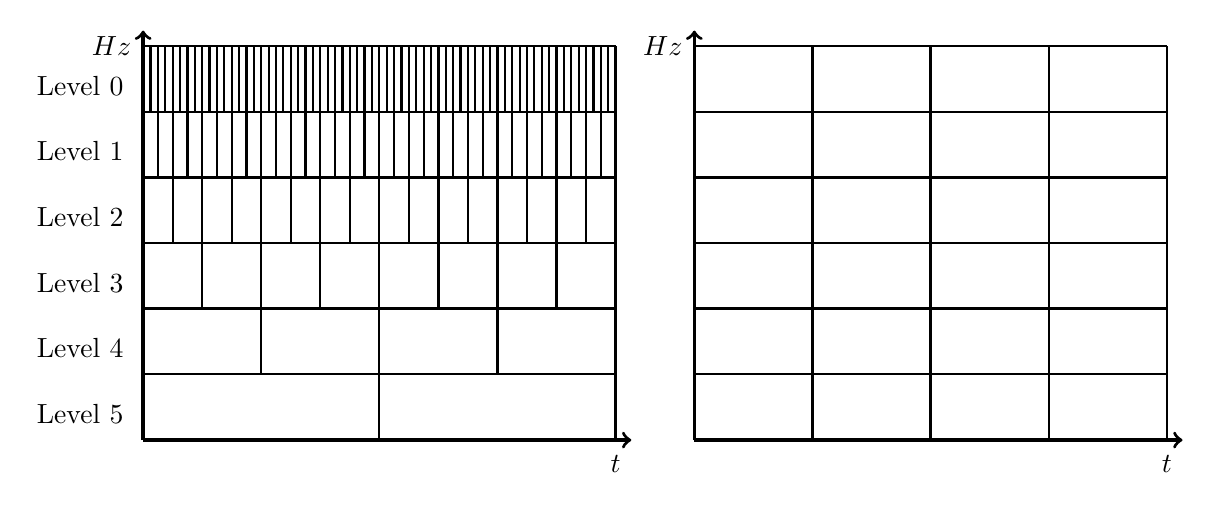
\begin{tikzpicture}
		\draw (6,-5.3) node{$t$};
		\draw (-0.4,0) node{$Hz$};
		
		\draw (-0.8,-0.5) node{Level 0};
		\draw (-0.8,-1.333) node{Level 1};
		\draw (-0.8,-2.166) node{Level 2};
		\draw (-0.8,-2.999) node{Level 3};
		\draw (-0.8,-3.832) node{Level 4};
		\draw (-0.8,-4.665) node{Level 5};
		
		
		\draw[->, very thick] (0,-5)--(0,0.2);
		\draw[->, very thick] (0,-5)--(6.2,-5);
		
		\draw[thick] (0,-0)--(6,-0);
		\draw[thick] (0,-0.833)--(6,-0.833);
		\draw[thick] (0,-1.666)--(6,-1.666);
		\draw[thick] (0,-2.499)--(6,-2.499);
		\draw[thick] (0,-3.33)--(6,-3.33);
		\draw[thick] (0,-4.166)--(6,-4.166);
		
		\draw[thick] (3,-5)--(3,0);
		\draw[thick] (6,-5)--(6,0);
		\draw[thick] (1.5,-4.166)--(1.5,0);
		\draw[thick] (4.5,-4.166)--(4.5,0);
		
		\draw[thick] (0.75,-3.33)--(0.75,0);
		\draw[thick] (2.25,-3.33)--(2.25,0);
		\draw[thick] (3.75,-3.33)--(3.75,0);
		\draw[thick] (5.25,-3.33)--(5.25,0);
		
		\foreach \x in {0,0.375,...,6}
		\draw[thick] (\x,-2.499)--(\x,0);
		
		\foreach \x in {0,0.1875,...,6}
		\draw[thick] (\x,-1.666)--(\x,0);
		
		\foreach \x in {0,0.09375,...,6}
		\draw[thick] (\x,-0.833)--(\x,0);
		
		\draw (13,-5.3) node{$t$};
		\draw (6.6,0) node{$Hz$};
		\draw[->, very thick] (7,-5)--(7,0.2);
		\draw[->, very thick] (7,-5)--(13.2,-5);
		
		\draw[thick] (7,-0)--(13,-0);
		\draw[thick] (7,-0.833)--(13,-0.833);
		\draw[thick] (7,-1.666)--(13,-1.666);
		\draw[thick] (7,-2.499)--(13,-2.499);
		\draw[thick] (7,-3.33)--(13,-3.33);
		\draw[thick] (7,-4.166)--(13,-4.166);
		
		\draw[thick] (8.5,-5)--(8.5,0);
		\draw[thick] (10,-5)--(10,0);
		\draw[thick] (11.5,-5)--(11.5,0);
		\draw[thick] (13,-5)--(13,0);
		\end{tikzpicture}
	}
	\caption{Multiskalenanalyse Auflösung im Vergleich zu STFT Analyse}\label{fig:faauf}
	
\end{figure}

\subsection{Analyse mit Frames}
In diesem Unterkapitel wird beschrieben welchen ablauf gewählt wurde um eine Analyse eines Testsignales durchzuführen.\\
Zuerst wurde ein Testsignal $x(t)$ erstellt. In der Grafik \ref{fig:frame-testsig} ist $x(t)$ abgebildet. Das Signal $x(t)$ besteht aus fünf verschiedenen Sinusschwingungen die aneinander gekoppelt wurden. Dazu eine kurze Beschreibung welche Frequenzen im dem Signal erhalten sind:\\
Die ersten zwei Ausschwenker schwingen über die dauer von jeweils $100$\text{ms}, mit der Frequenz 110 \text{[Hz]}. \\
Der dritte Ausschwenker schwingt $100$\text{[ms]} mit $220\cdot 2^{\frac{1}{12}}$\text{[Hz]}, folgend auf einen $100$\text{[ms]} Ausschwenker mit einer Frequenz von $220\cdot 2^{\frac{2}{12}}$ \text{[Hz]}. \\
Der letzte Block beginnt mit $220\cdot 2^{\frac{2}{12}}$\text{[Hz]} über eine dauer von $100$\text{[ms]} bis die Amplitude $a=1$ erreicht ist. Danach wechselt das Signal fliessend auf $220\cdot 2^{\frac{5}{12}}$\text{[Hz]} für $100$\text{[ms]} und endet mit $220\cdot 2^{\frac{6}{12}}$\text{[Hz]}. Die gesamte Signaldauer ist genau eine Sekunde lang. \\



In der Grafik \ref{fig:Frame-Analyse} wird eine Frame-Analyse und eine cwt-Analyse des gleichen Testsignales\ref{fig:frame-testsig} nebeneinander gestellt. Darin kann mun nun die unterschiede 
\begin{figure}[!ht]
	\centering
	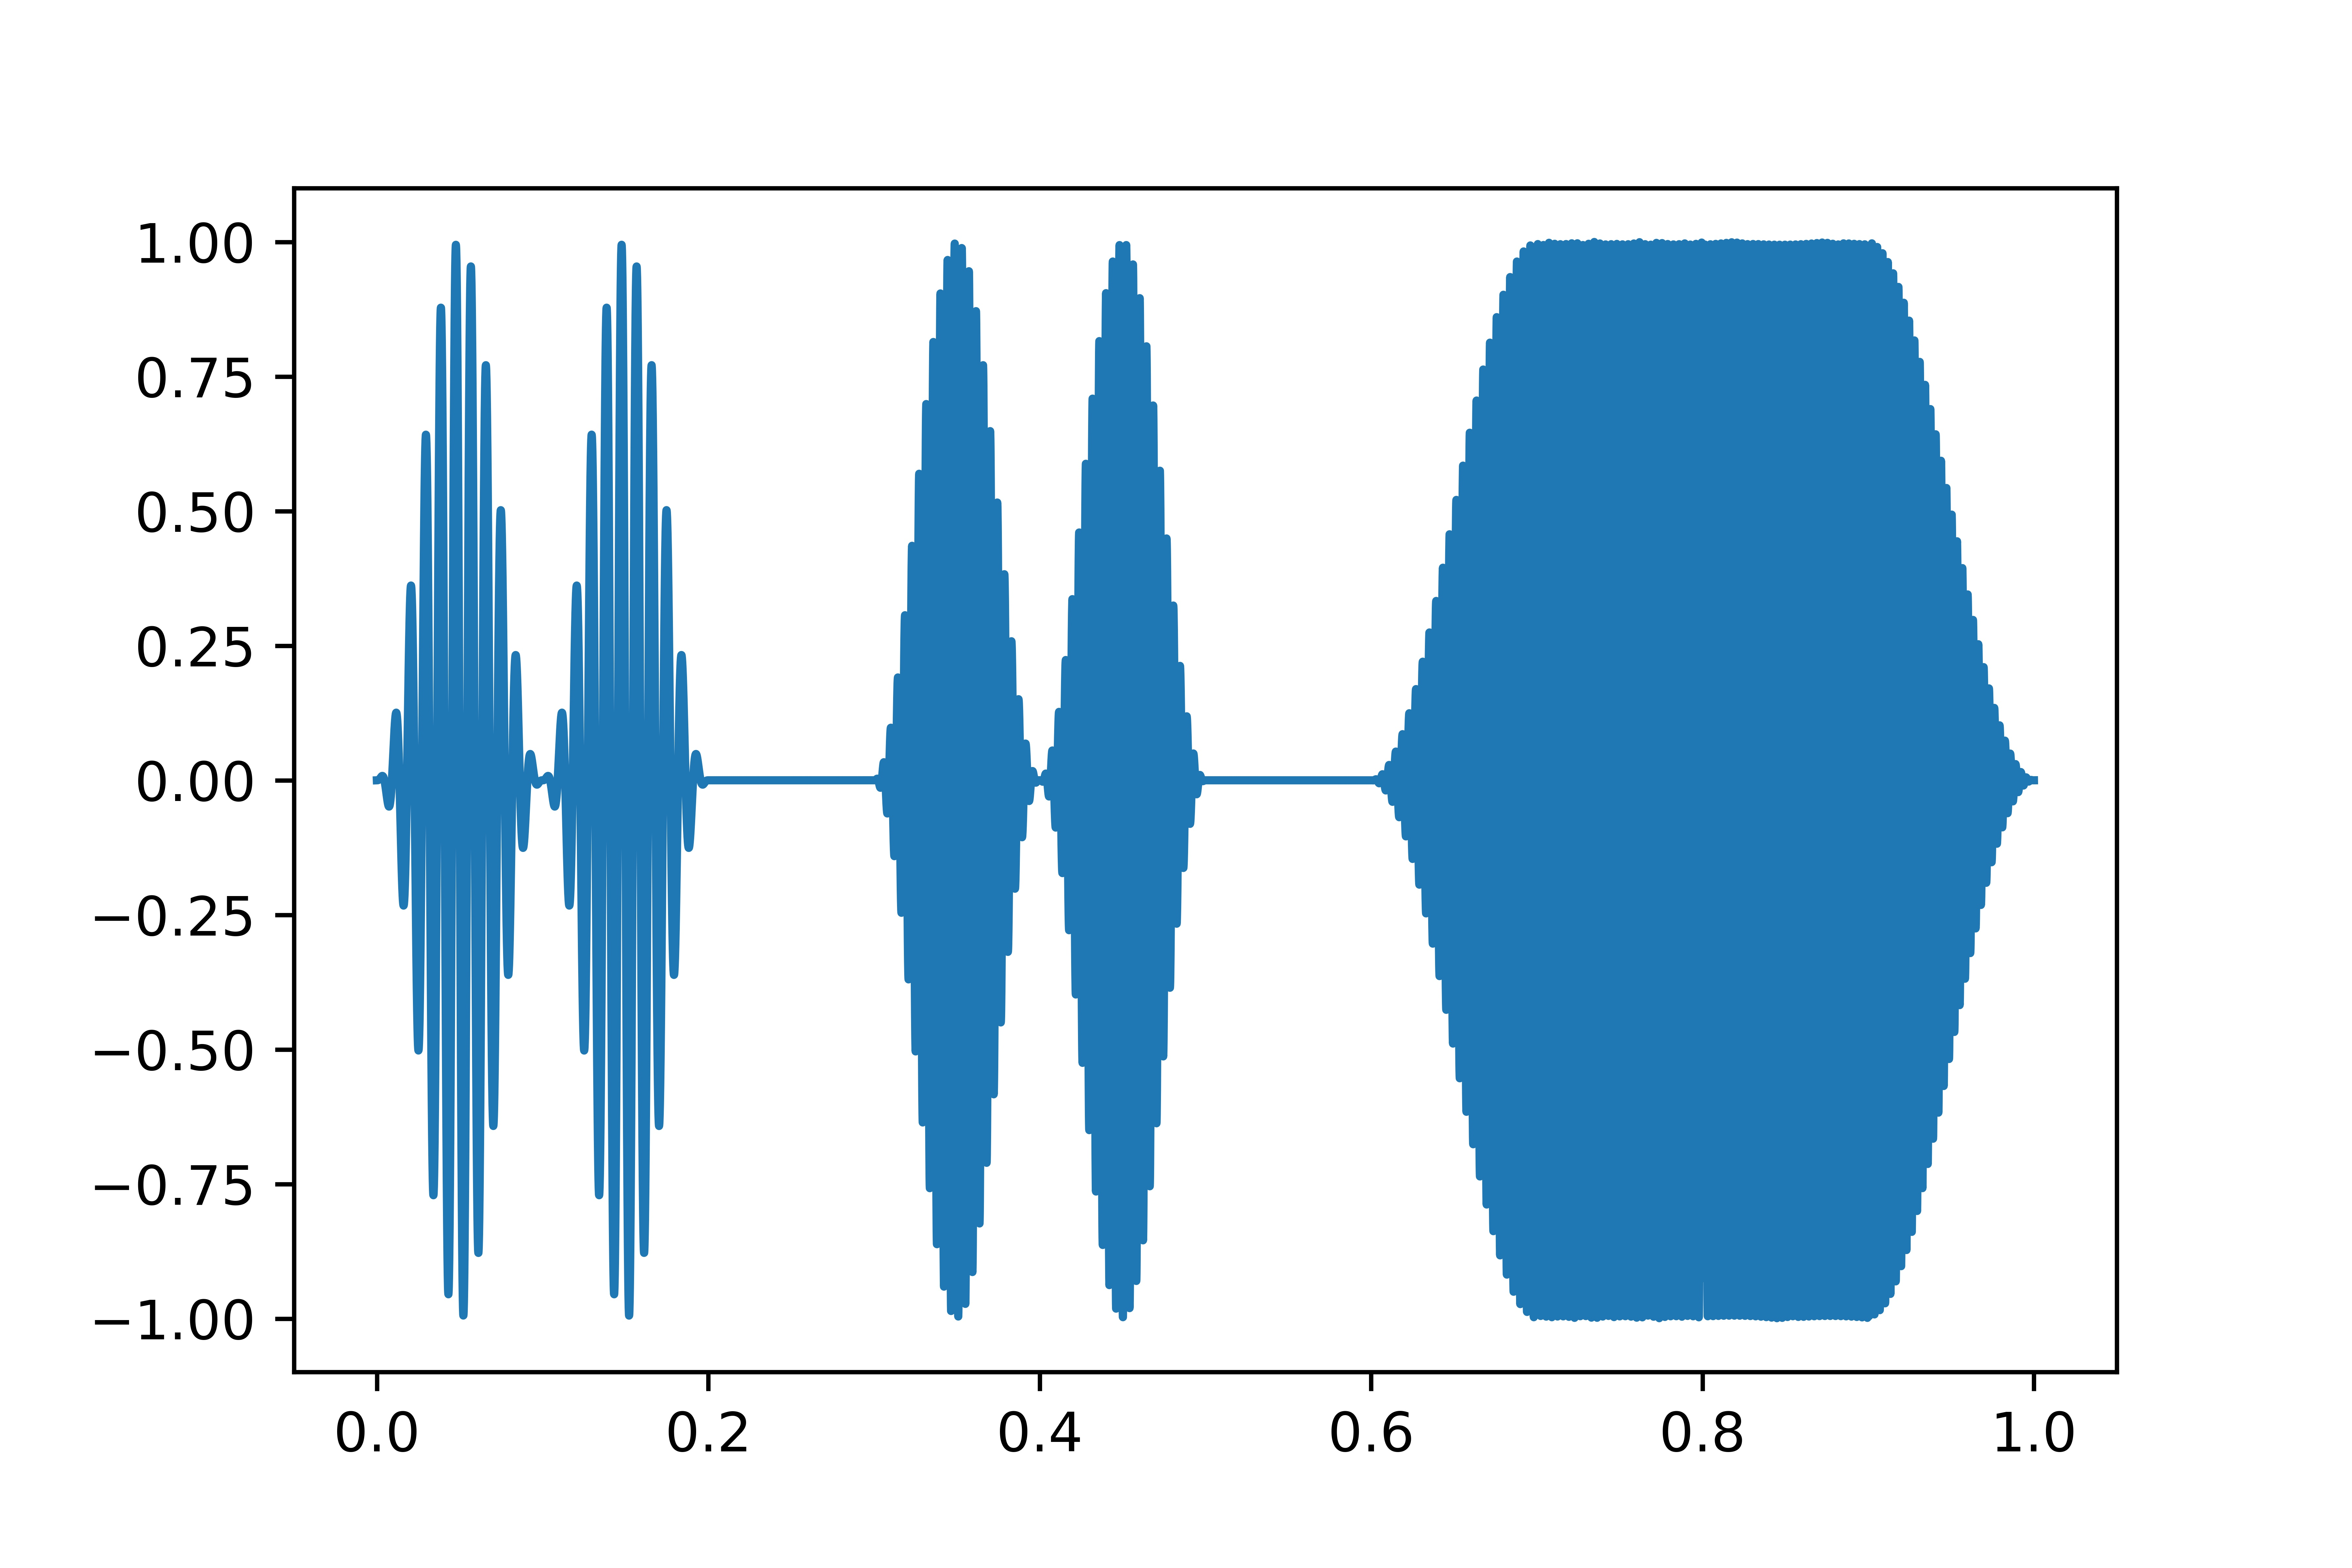
\includegraphics[width=\linewidth]{papers/autotune/sections/frames/images/testsig.jpg}
	\captionof{figure}{Testsignal}\label{fig:frame-testsig}
	\begin{tabularx}{\columnwidth}{XX}
		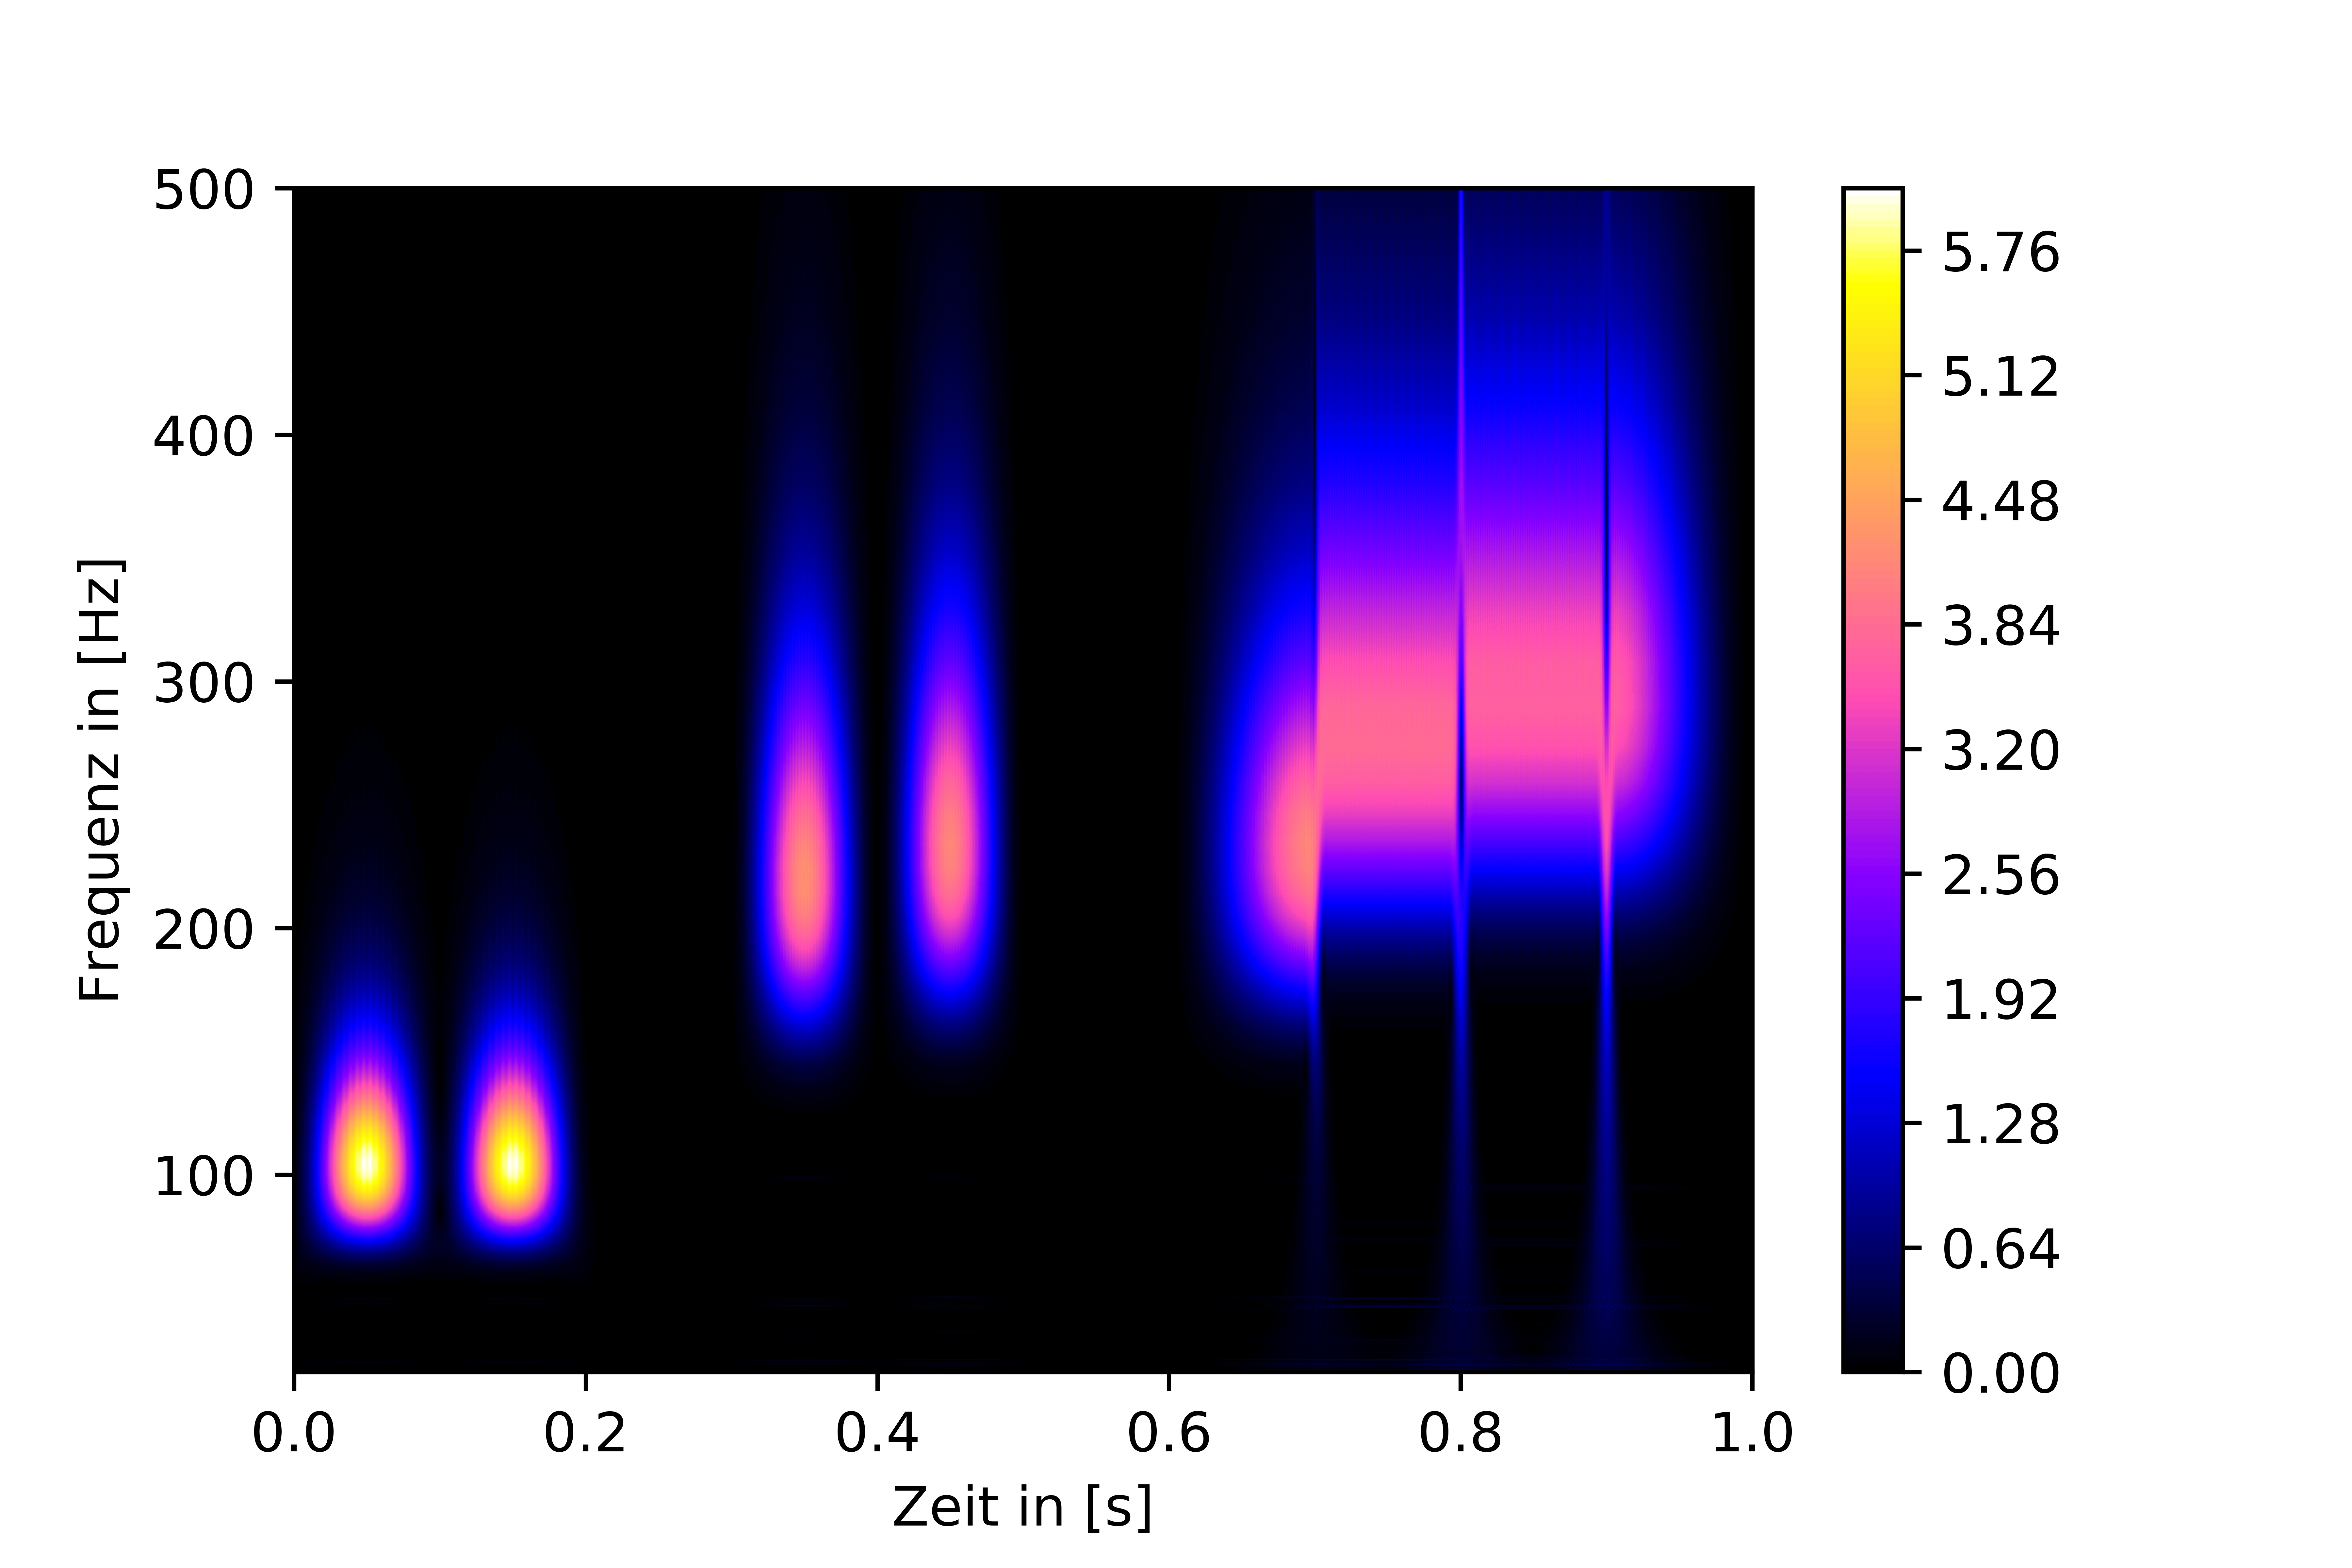
\includegraphics[width=1.3\linewidth]{papers/autotune/sections/frames/images/cwt.jpg}
		\captionof{figure}{Cwt Analyse mit komplexem Gauss Wavelet des Testsignal}\label{fig:stft256}
		&   \includegraphics[width=1.3\linewidth]{papers/autotune/sections/frames/images/12dwt.jpg}   
		\captionof{figure}{Dauberchi 8 Frame Analyse des Testsignal}\label{fig:cwtsweep}         
	\end{tabularx}
	\caption{Vergleich der Absolutwerte von der cwt und der Frame Analyse mit 12 Basen}
	\label{fig:Frame-Analyse}
\end{figure}%

\begin{figure}[!ht]
	\centering
	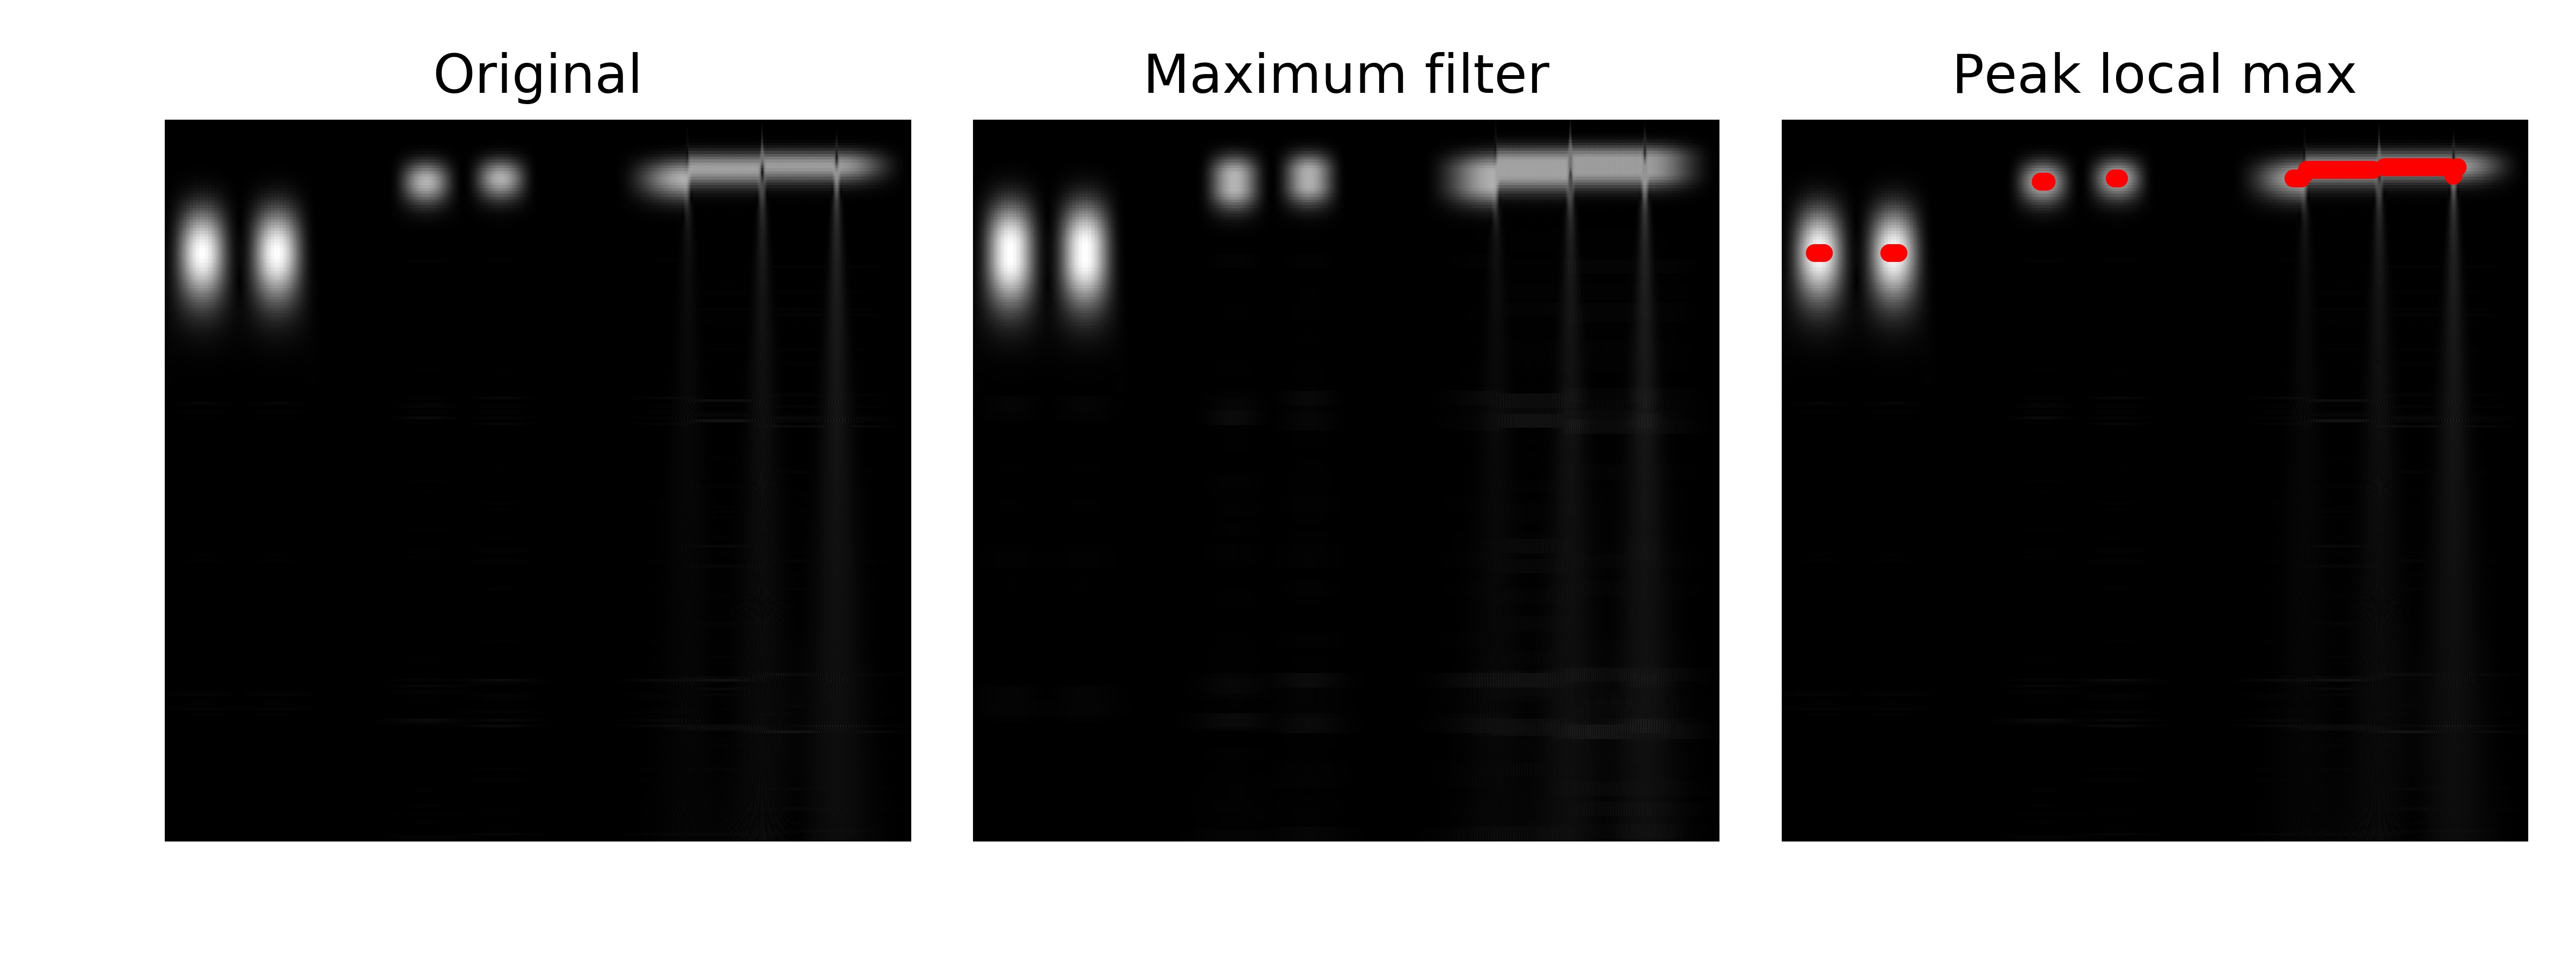
\includegraphics[width=\linewidth]{papers/autotune/sections/frames/images/cwtmaxima.jpg}
	\captionof{figure}{Maxima berechnung  des CWT}\label{fig:cwt:max}
\end{figure}%

\begin{figure}[!ht]
	\centering
	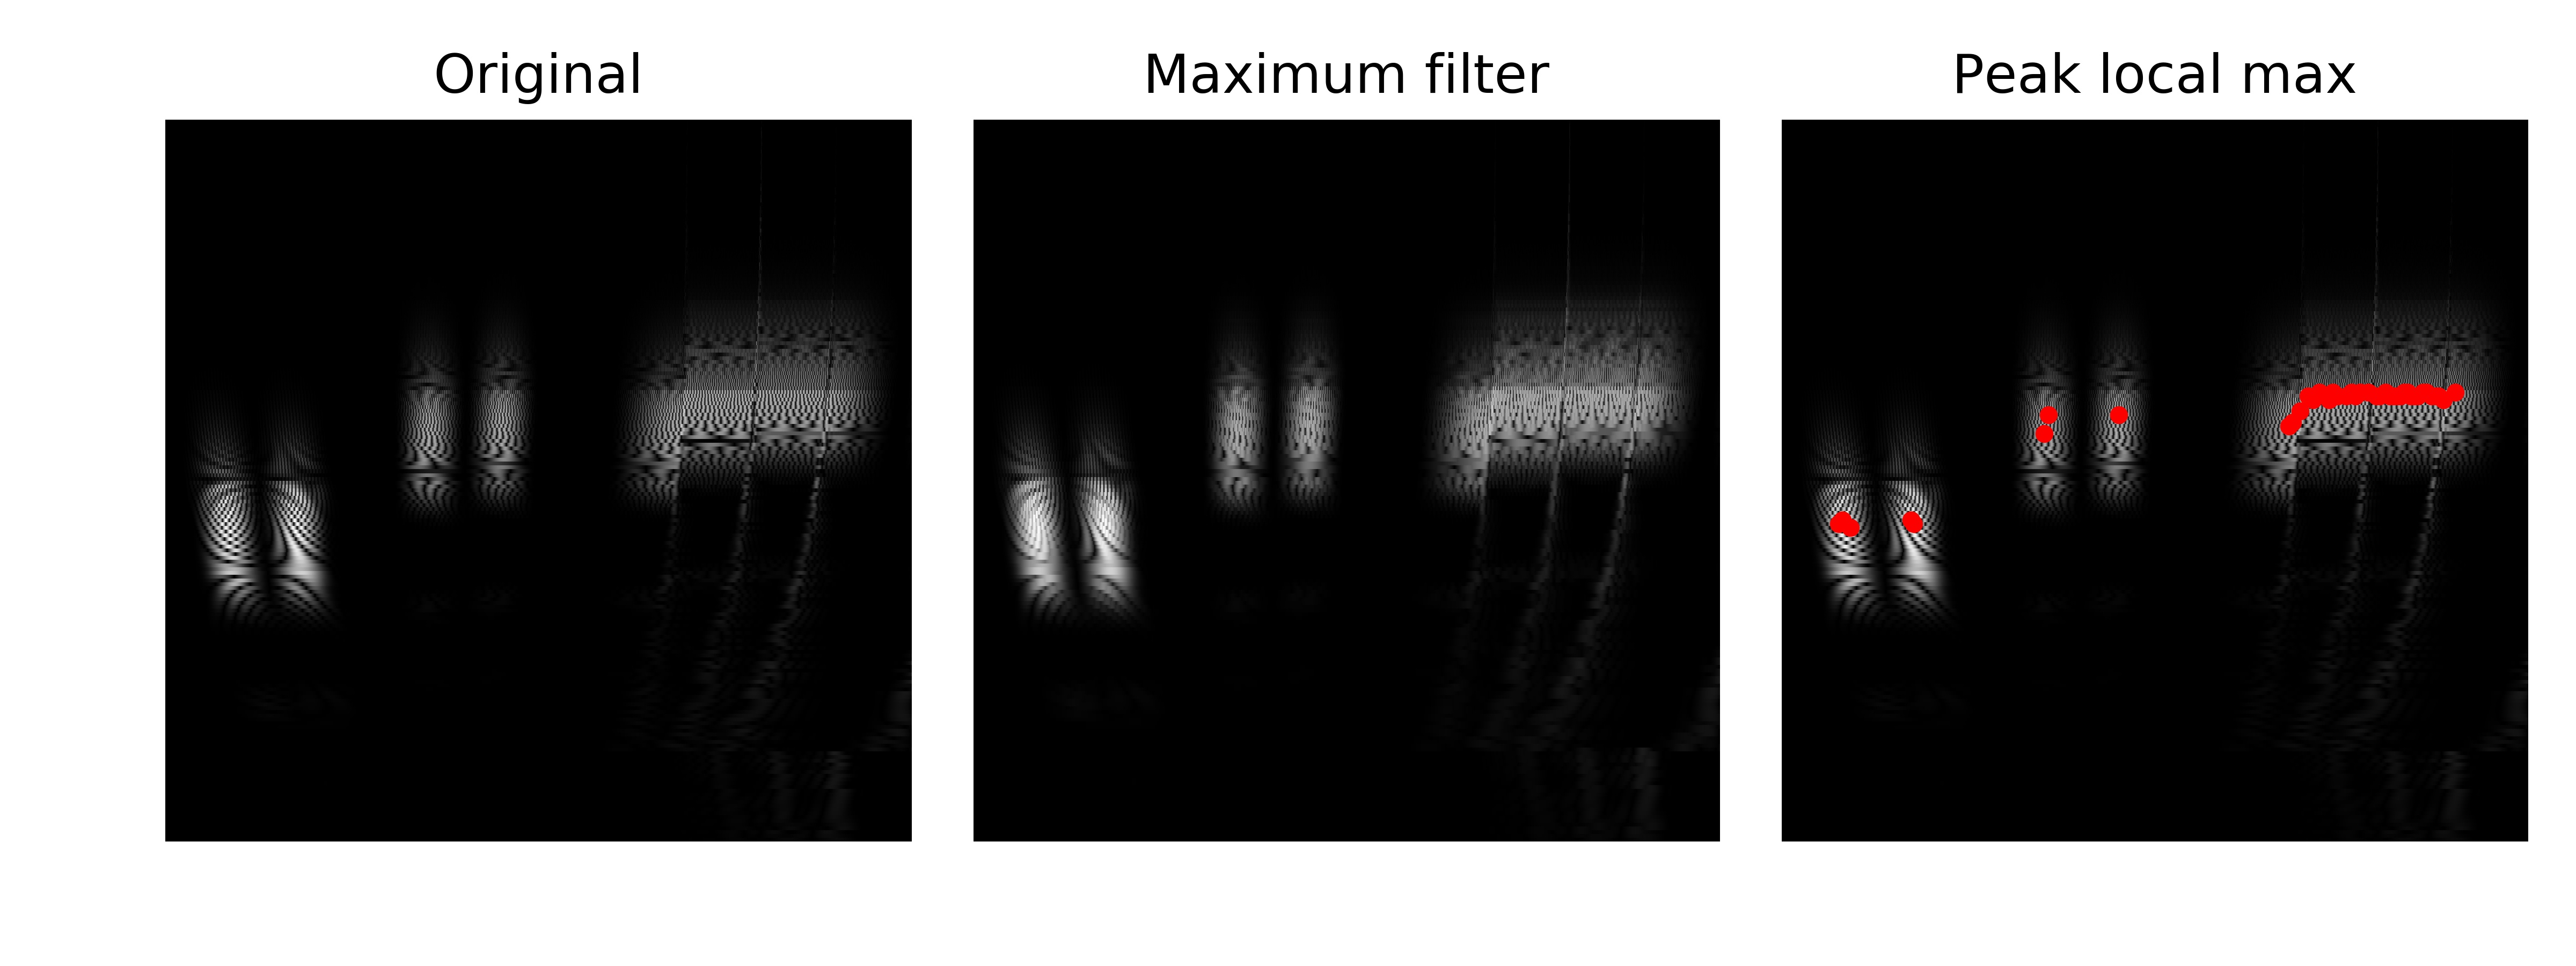
\includegraphics[width=\linewidth]{papers/autotune/sections/frames/images/dwtmaxima.jpg}
	\captionof{figure}{Maxima berechnung  des DWT}\label{fig:cwt:max}
\end{figure}%


